\chapter{Logística del proyecto}

En este capítulo se recogen todos los aspectos logísticos del proyecto, tales como ciclo de vida, planificación y presupuestos y costes.

\section{Ciclo de vida}

El ciclo de vida de este proyecto ha sido el siguiente:
\begin{enumerate}
\item[0.] \textbf{Documentación sobre el mundo matemático del póker:} En esta fase previa a la fase inicial inicial,ha consistido en reunir informaicón sobre el juego de póker, las bases matemáticas del póker, los estudios de inteligencia artificial y de juego digital de póker. Esta fase es previa a las demás fases, pues es necesario tener unas bases de conocimiento so
\item \textbf{Determinación de objetivos y planificación:} En esta fase, se plantearon los objetivos, pues habían varias posibilidades en torno al objeto de estudio dentro del juego de póker y la matemática, así como plantear una planificación.
\item \textbf{Diseño del proyecto}: Con los objetivos definidos, se tomó el diseño del simulador de póker, se planteó que el algoritmo fuera una caja negra y se empezaron a tomar las decisiones y abstracciones para intentar suplir dificultades (Como limitar a 2 el número de jugadores)
\item \textbf{Desarrollo del código}: En este punto, se empezó a hacer el desarrollo del software. El motor de juego fue el primero en empezar a ser desarrollado, ya que era una base para poder hacer funcionar el algoritmo, auqnue se empezaron a desarrollar cosas del algoritmo, pero en fases muy tempranas. Una vez el motor de juego fue funcional (con las funciones correspondientes al algoritmo sustituidas por otras temporalmente) se centraron los recursos en el software del algoritmo
\item \textbf{Pruebas de código}: Si bien las pruebas de código son un elemento indisppensable para la vida del proyecto y se tendrían que ejecutar desde que se tiene una versión muy primitiva del software, en este caso se tuvo que esperar hasta que el motor de juego estuviera bastante avanzado para poder empezar a hacer pruebas, de manera similar como paraba con las pruebas individuales del algoritmo. Sin embargo, el funcionamiento como un solo elemento de motor de juego y algoritmo no es posible hacerlo hasta que la conexión entre ambos es plenamente funcional.
\item \textbf{Toma de datos y evidencias}: una vez teniendo las pruebas de código hechas y, habiendo copmrobado la funcionalidad del software en conjunto, se puede proceder a la toma de datos, en las que se ejecuta el conjunto del software y se obtienen registros con los resultados de las iteraciones del juego automático del software.
\end{enumerate}

Además de estas fases secuenciales, hay una fase del proyecto que se desarrolla en paralelo con el resto del document, y es la documentación del proceso y del proyecto, pues esta fase es necesaria para poder formalizar el trabajo realizado, documentando todas las acciones realizadas a lo largo del proceso.

\section{Planificación}

La planificación de este proyecto ha sido bastante turbulenta, principalmente por la diferencia entre la planificación inicial y la planificación final.

\subsection{Planificación inicial}

La planificación inicial del proyecto fue comenzar el proyecto en octubre y terminarlo en enero siguiendo, de manera aproximada, el diagrama de Gantt\footnote{Un diagrama de Gantt\cite{gantt} es un diagrama utilizado en la planificación de los proyectos, cuya finalidad es mostrar una vista general de la planificación de todas las tareas. Este diagrama muestra la fecha de inicio y finalización del proyecto, las tareas de dicho proyecto (con sus respectivas fechas programadas de inicio y final, asi como su duración estimada), la distribución de personas (en caso de que haya varias personas) y la relación entre las tareas.} de la figura \ref{fig:gant1}.
\begin{figure}[tb]
\centering
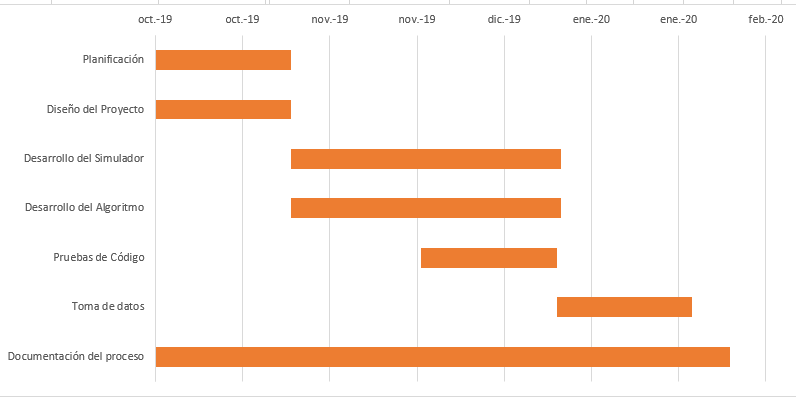
\includegraphics[width=0.6\textwidth]{figuras/gant1.png}   
\caption{Diagrama de Gantt de la planificación inical del proyecto}
\label{fig:gant1}
\end{figure}

Esta planificación inicial fue demasiado ambiciosa, sin tener en consideración la situación y la disponibilidad de recursos durante ese periodo planificado, lo que desembocó en la imposibilidad de cumplir esta planificación y tener que replantear toda la planificación.

\subsection{Planificación final}

Una vez que la planificación inicial del proyecto fue totalmente inviable, fue necesario restablecer la planificación del proyecto. La planificación final ha sido más realista, salvando las distancias con las demoras sufridas a raiz de acontecimientos de gran importancia en la vida cotidiana.

El diagrama de la planificación final es el diagrama de la figura \ref{fig:gant2}.

\begin{figure}[tb]
\centering
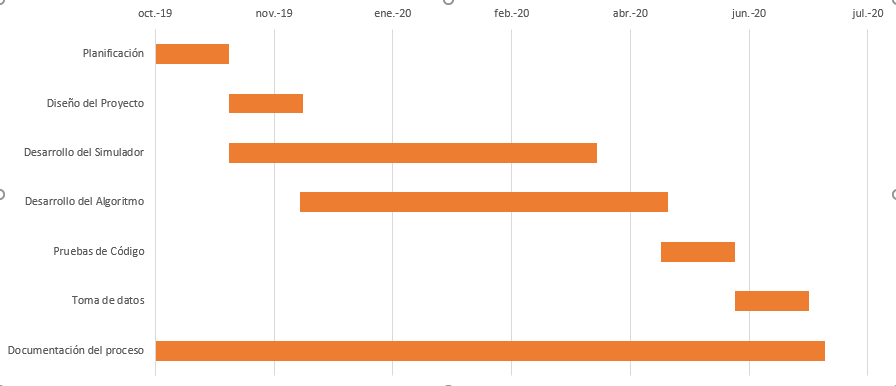
\includegraphics[width=0.6\textwidth]{figuras/gant2.png}   
\caption{Diagrama de Gantt de la planificación final del proyecto}
\label{fig:gant2}
\end{figure}

\section{Presupuesto}

Si bien no había una planificación sobre presupuesto a gastar ya que, al ser un proyecto de programación, no había previsión de realizar gastos económicos, algunos gastos económicos si que hubo.

\subsection{Material}
Al principio, no había ningún tipo de planteamiento de hacer gasto económico para este proyecto. Pero las necesidades a la que fue avanzando el proyecto cambiaron, y fue necesario disponer de los siguientes elementos:
\begin{itemize}
\item Una baraja francesa de póker. Si bien esto puede parecer algo básico e, incluso, innecesario, la adquisición de un kit de poker contribuyó bastante, sobre todo en las fases iniciales del proyecto, pues servía de ayuda visual para la codifcación del funcionamiento de una ronda de juego de Texas Hold'em. Debido a que fue utilizada principalmente en momentos de atasco de ideas, acabó convirtiéndose en una ayuda para la concentración.
\item Hold'em Excellence (English Edition). Debido a la dificultad de encontrar fuentes y bibliografía en torno a la fórmula de Chen, fue necesaria la adquisición del libro donde se definió por primera vez por Lou Krieger. \cite{krieger}.
\end{itemize}

Además de ello, los gastos a lo largo del proyecto en dosisfuertes de cafeína para poder aprovechar el tiempo al máximo al compaginar demasiadas cosas.

%\subsection{Personal}

%Si bien el proyecto no tenía intención de causar gasto personal, acabó generando mucho agotamiento y estrés, especialmente en las fechas de cumplimieto de la planificación (con mayor intensidad en la planificación inicial que en la final), que acabó provocando en privaciones largas de sueño.

\subsection{Resumen de costes}

\begin{longtable}[c]{ll|l|l|}
\hline
\rowcolor{lightgray}\multicolumn{1}{|l|}{\textbf{Elemento}} & \textbf{Cantidad} & \textbf{Coste unitario} & \textbf{Coste} \\ \hline
\multicolumn{1}{|l|}{\textit{Kit de Poker}} & 1 & 10 & 10 \\ \hline
\multicolumn{1}{|l|}{\textit{Hold'em Excelence (Kindle Edition)}} & 1 & 8,54 € & 8,54 € \\ \hline
 &  & \textbf{Total} & \textbf{18,54} \\ \cline{3-4} 

\end{longtable}